\documentclass[paper=a4, fontsize=11pt]{scrartcl}
\usepackage[T1]{fontenc}
\usepackage{fourier}

\usepackage[english]{babel}															% English language/hyphenation
\usepackage[protrusion=true,expansion=true]{microtype}	
\usepackage{amsmath,amsfonts,amsthm} % Math packages
\usepackage[pdftex]{graphicx}	
\usepackage{url}
\usepackage{gensymb}


%%% Custom sectioning
\usepackage{sectsty}
\allsectionsfont{\centering \normalfont\scshape}


%%% Custom headers/footers (fancyhdr package)
\usepackage{fancyhdr}
\pagestyle{fancyplain}
\fancyhead{}											% No page header
\fancyfoot[L]{}											% Empty 
\fancyfoot[C]{}											% Empty
\fancyfoot[R]{\thepage}									% Pagenumbering
\renewcommand{\headrulewidth}{0pt}			% Remove header underlines
\renewcommand{\footrulewidth}{0pt}				% Remove footer underlines
\setlength{\headheight}{13.6pt}

\numberwithin{equation}{section}		% Equationnumbering: section.eq#
\numberwithin{figure}{section}			% Figurenumbering: section.fig#
\numberwithin{table}{section}				% Tablenumbering: section.tab#


%%% Maketitle metadata
\newcommand{\horrule}[1]{\rule{\linewidth}{#1}} 	% Horizontal rule

\title{
		%\vspace{-1in} 	
		\usefont{OT1}{bch}{b}{n}
		\normalfont \normalsize \textsc{BITS PILANI K K BIRLA GOA CAMPUS} \\ [25pt]
		\horrule{0.5pt} \\[0.4cm]
		\huge A Fuzzy Logic Controller for Position Control of a Stepper Motor Using MATLAB and Simulink \\
		\horrule{2pt} \\[0.5cm]
}
\author{
		\normalfont 								\normalsize
        RR SREEKRISHNA\\[-3pt]
        2012A3PS180G\\[-3pt]		\normalsize
        \today
}
\date{}

%%% Begin document
\begin{document}
\maketitle
\indent \section{Introduction}
This is a report for the design of a Fuzzy Logic Controller using Simulink and MATLAB.This controller is for the position control of different motors. I have chosen a DC Motor, Stepper Motor and a Picomotor for the purposes of Simulation.Any motor can be incorporated in the design. The differentiating characteristics of every motor is clearly depicted in this report. For a stepper motor, one of the most important parameter is its step angle. Common step sizes are 1.8\degree, 2.5\degree, 7.5\degree, 15\degree.In this work I have chosen the step size as 1.8\degree.\\
\indent There are various methods offered in literature for controlling motors. Most Common being PID Controllers. However it is seen that PID like fuzzy controllers perform better than the conventional controllers. It is also shown that even without knowing the  details of the control system we can construct a Fuzzy Logic Controller based on the experience about the Position Controller. Recently much more emphasis is given to the designing of PID like Fuzzy controllers. \\

\subsection{Overview of the System}
\begin{figure}[ht!]
\centering
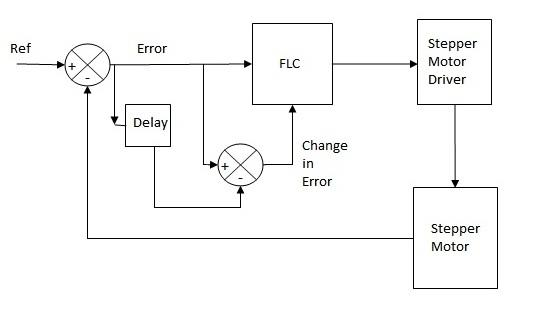
\includegraphics[width=90mm]{system_overview_stepper.jpg}
\caption{Block Diagram of the Proposed System \label{overflow}}
\end{figure}
In this system our aim is to keep the motor in the same position as given by the PSD (Position Sensor Detector). This implies that the error has to be reduced to zero as the system moves towards its desired position given by the reference position. There are two controllers designed for the purpose of comparison. First one is a conventional PID Controller For the Fuzzy Logic Controller there are three main stages involved in designing the Controller namely \begin{itemize}\item1. Fuzzification - Conversion of Crisp Sets into Fuzzy Sets. \item2. Infe
\subsubsection{Heading on level 3 (subsubsection)}

\paragraph{Heading on level 4 (paragraph)}


\section{Lists}

\subsection{Example for list (3*itemize)}
\begin{itemize}
	\item First item in a list 
		\begin{itemize}
		\item First item in a list 
			\begin{itemize}
			\item First item in a list 
			\item Second item in a list 
			\end{itemize}
		\item Second item in a list 
		\end{itemize}
	\item Second item in a list 
\end{itemize}

\subsection{Example for list (enumerate)}
\begin{enumerate}
	\item First item in a list 
	\item Second item in a list 
	\item Third item in a list
\end{enumerate}
%%% End document
\end{document}